\documentclass[]{article}

\usepackage{color}

\usepackage{mathtools}
\usepackage{amsmath}
\usepackage{amssymb}
\usepackage{hyperref}
\usepackage{xcolor}
\usepackage{subcaption}
\usepackage{svg}
\usepackage[utf8]{inputenc}
\usepackage[english]{babel}

\usepackage{tikz}
\usetikzlibrary{shapes.geometric, arrows}
\tikzstyle{startstop} = [rectangle, rounded corners, minimum width=3cm, minimum height=1cm,text centered, draw=black, fill=red!30]
\tikzstyle{io} = [trapezium, trapezium left angle=70, trapezium right angle=110, minimum width=3cm, minimum height=1cm, text centered, draw=black, fill=blue!30]
\tikzstyle{process} = [rectangle, minimum width=3cm, minimum height=1cm, text centered, draw=black, fill=orange!30]
\tikzstyle{decision} = [diamond, minimum width=3cm, minimum height=1cm, text centered, draw=black, fill=green!30]
\tikzstyle{arrow} = [thick,->,>=stealth]

\hypersetup{
    colorlinks,
    linkcolor={black},
    citecolor={black},
    urlcolor={black}
}

\title{Analyzing and composing music with algorithms and machine learning}
\author{
    \begin{tabular}{rl}
        \normalsize{Author: } & \normalsize{Dimo Chanev} \\
        \scriptsize{Supervisiors: } & \scriptsize{Emil Kelevedjiev}\\
                                    & \scriptsize{Zornitsa Dzhenkova}
    \end{tabular}
}

\begin{document}
    \maketitle
    \newpage

    \tableofcontents

    \newpage
    \begin{abstract}
        The goal of the project is to compare, experiment and proove some mathematical algorithms for analyzing music and composing a similar pieces of music with random numbers. The algorithms are based on analyzing some relations from given note notations of given melodies, in form of standart MIDI files.
    \end{abstract}

    \newpage

    \section{Introduction}
        \subsection {Frequency relations (tuning)}
        \paragraph{} The sound is type of mechanical vibration (waves) so it has the parameters of all the normal mechanical waves. However in the field of music we are most interested in the frequency of the wave, because it makes the variety of tones we hear. But not every sequence of frequencies sounds pleasent to the human. So the people developed some algorithms to ``syncronize'' the sequence of tunes. Here are the most used of them:

            \subsubsection {Pythagorean tuning} 
            \paragraph{} The Pythagorean tuning is the base of almost all tuning sysytems. It is based on the Pythagorean fractions.\\
                \begin{figure}[h]
                    $$f = \frac{i + 1}{i} ;\ i = 1, 2, ..., n$$
                    \caption{Pythagorean fractions}
                \end{figure}\paragraph{}
                It is assumed that if the frequencies corelate like these numbers, we hear them in harmony and the music will sound pleasent (if we select appropriate sequence of these tones of course).\paragraph{}
                If we pick a string with given length we know that the frequency of the produced sound depends on the length of the string. So to pick the ``perfect'' fraction we have to devide it like the Pythagorean fractions.
                \begin{figure}[h]
                    \begin{center}
                        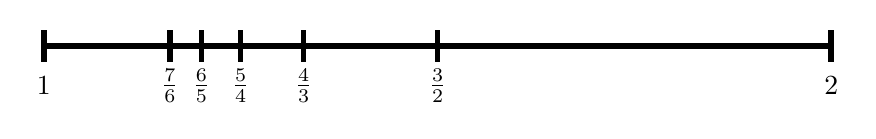
\begin{tikzpicture}
                            \draw [line width = 2] (0, 0) -- (10, 0);
                            \draw [line width = 2] (0, 0.2) -- (0, -0.2);
                            \draw (0, -0.5)node {$1$};
                            \draw [line width = 2] (10, 0.2) -- (10, -0.2);
                            \draw (10, -0.5)node {$2$};
                            \draw [line width = 2] (5, 0.2) -- (5, -0.2);
                            \draw (5, -0.5)node {$\frac{3}{2}$};
                            \draw [line width = 2] (3.3, 0.2) -- (3.3, -0.2);
                            \draw (3.3, -0.5)node {$\frac{4}{3}$};
                            \draw [line width = 2] (2.5, 0.2) -- (2.5, -0.2);
                            \draw (2.5, -0.5)node {$\frac{5}{4}$};
                            \draw [line width = 2] (2, 0.2) -- (2, -0.2);
                            \draw (2, -0.5)node {$\frac{6}{5}$};
                            \draw [line width = 2] (1.6, 0.2) -- (1.6, -0.2);
                            \draw (1.6, -0.5)node {$\frac{7}{6}$};
                        \end{tikzpicture}
                        \caption{The ``pefect'' string separation}            
                    \end{center}
                \end{figure}

            \subsubsection{Equal temperament}
            \paragraph{}Equal temperament is a tuning scale developed by Vincenzo Galilei. His idea is that the frequency ratio between each pair of ajacent notes is the same. In equal temperament tunings, the generating interval is often found by dividing some larger desired interval into a number of smaller equal steps (equal frequency ratios between neighbouring notes). The tones are devided in groups called octaves. The ratio between the frequencies of last and the first tone of the octave is two.
                $$\frac{last\ tune}{first\ tune} = \frac{2}{1}$$ \paragraph{}
                In the Western music, the most commonly used tunning system since the 18th century has been the twelve-tone equal temperament(or 12-TET). The 12-TET devides the octave in 12 eqal parts, all of them eqal on logaritmic scale, with ratio $\sqrt[12]{2} = 2^\frac{1}{12} \approx 1.05946$. In modern times 12-TET is usually tunned relatively to the standart frequency of 440 Hz, called A4, meaning that the note A is tuned to 440 Hz and all other note are derived by the logaritmic scale described above. \paragraph{}
                Equal temperament is an approximation of the Pythagorean scale, which is more convinient for use.\\
                \begin{figure}[h]
                    \begin{center}
                        \begin{tabular}{| l | l | l | l |}
                            \hline
                            \textbf{Name} & \textbf{12-TET} & \textbf{Pythagorean scale}\\\hline
                            Unision ($C$) & $2^\frac{0}{12} = 1$ & $\frac{1}{1} = 1$ \\ \hline
                            Minor second ($C\sharp/D\flat$) & $2^\frac{1}{12} \approx 1.05946$ & $\frac{16}{15} \approx 1.06666$\\ \hline
                            Major second ($D$) & $2^\frac{2}{12} \approx 1.12246$ & $\frac{9}{8} = 1.125$ \\ \hline
                            Minor third ($D\sharp/E\flat$) & $2^\frac{3}{12} \approx 1.18920$ & $\frac{6}{5} = 1.2$ \\ \hline
                            Major third ($E$) & $2^\frac{4}{12} \approx 1.25992$ & $\frac{5}{4} = 1.25$ \\ \hline
                            Perfect fourth ($F$) & $2^\frac{5}{12} \approx 1.33484$ & $\frac{4}{3} \approx 1.33333$ \\ \hline
                            Tritone ($F\sharp/G\flat$) & $2^\frac{6}{12} \approx 1.41421$ & $\frac{7}{5} = 1.4$* \\ \hline
                            Perfect fifth ($G$) & $2^\frac{7}{12} \approx 1.49830$ & $\frac{3}{2} = 1.5$ \\ \hline
                            Minor sixth ($G\sharp/A\flat$) & $2^\frac{8}{12} \approx 1.58740$ & $\frac{8}{5} = 1.6$* \\ \hline
                            Major sixth ($A$) & $2^\frac{9}{12} \approx 1.68179$ & $\frac{5}{3} \approx 1.66666$* \\ \hline
                            Minor seventh ($A\sharp/B\flat$) & $2^\frac{10}{12} \approx 1.78179$ & $\frac{16}{9} \approx 1.77777$* \\ \hline
                            Major seventh ($B$) & $2^\frac{11}{12} \approx 1.88774$ & $\frac{15}{8} = 1.875$* \\ \hline
                            Octave ($C$) & $2^\frac{12}{12} = 2$ & $\frac{2}{1} = 2$ \\ \hline
                            \multicolumn{3}{c}{Note: the values with * can't be represented like Pythagorean fractions with decent accuracy}\\
                            \multicolumn{3}{c}{but the human ear can't differentiate this (in the most cases).}\\
                        \end{tabular}
                        \caption{Values of the tones in 12-TET and Pythagorean scale}
                    \end{center}
                \end{figure}
        \subsection {MIDI standart}
        \paragraph{} The purpose of MIDI is to define a way compact representation of musical sheets, which makes it appropriate for disk storage.\paragraph{}
            The standart MIDI(SMID) file is devided into chunks. Each chunk has a type and length represented as ASCII and 32 bit number respectively. There are two types of chunks: ``MThd''(e.g. Header chunk) and ``MTrk''(e.g. Track chunk). There is always one header while there can be more than one track.
            \subsubsection{Header chunk}
            \paragraph{}The header chunk contains data for the whole file. It has fixed length of 6 bytes. The first 2 bytes represent the format of file:
                \begin{itemize}
                    \item 0 $\to$ One track
                    \item 1 $\to$ Multiple tracks but one song
                    \item 2 $\to$ Multiple song
                \end{itemize}
                The second 2 bytes represent the number of tracks. For format 0 it is always 1. And the last two bytes represent how many ticks are in a quarter note.
            \subsubsection{Track chunks}
            \paragraph{}Each track is composed of events. Each event has delta time - the time (in ticks) which passes after the previous event before executing this event. There are two types of events: MIDI events - the ones which represent the actual music and META - these which supply additional info like titles, lyrics, etc. \paragraph{}
                Each MIDI event that has to play note uses this standart for encoding the frequency of the played tune:
                $$f = 440 * 2^\frac{d - 69}{12}\ where\ d\ is\ the\ note\ number\ and\ f\ is\ the\ frequency$$
                Therefore the note number is:
                $$d = 69 + 12\log_2 \frac{f}{440}$$
        \subsection{Markov chains}
        \paragraph{}Markov chain is a stochastic model which describes a sequence of events in which the probability of each event depends entierly on the previous event (in some cases the previous $n$ but the table which decribes the chain size becomes big quickly because it equals to $k^n\ where\ k\ is\ the\ number\ of\ events$).\paragraph{}
                Markov chains are represented as table in the most cases. Each cell of the table hold the probability of triggering an event from the row/collumn after the event in the collumn/row respectively (see Figure 4).
                \begin{figure}[h]
                    \begin{center}
                        
                        \begin{subfigure}[a]{0.4\textwidth}
                            \begin{tabular}{|c|c|c|c|}
                                \hline
                                & \multicolumn{3}{|c|}{Next event} \\ \cline{2-4}
                                & A & B & C \\ \hline
                                A & 33\% & 22\% & 45\% \\ \hline
                                B & 81\% & 9\% & 10\% \\ \hline
                                C & 30\% & 60\% & 10\% \\ \hline
                            \end{tabular}
                        \end{subfigure}
                        \begin{subfigure}[b]{0.4\textwidth}
                            \begin{tabular}{|c|c|c|c|c|}
                                \hline
                                \multicolumn{2}{|c|}{} & \multicolumn{3}{|c|}{Next event} \\ \cline{3-5}
                                \multicolumn{2}{|c|}{} & A & B & C \\ \hline
                                A & A & 16\% & 16\% & 68\% \\ \hline
                                A & B & 100\% & 0\% & 0\% \\ \hline
                                A & C & 12\% & 75\% & 13\% \\ \hline
                                B & A & 37\% & 25\% & 38\% \\ \hline
                                B & B & 0\% & 0\% & 100\% \\ \hline
                                B & C & 100\% & 0\% & 0\% \\ \hline
                                C & A & 33\% & 33\% & 34\% \\ \hline
                                C & B & 83\% & 17\% & 0\% \\ \hline
                                C & C & 100\% & 0\% & 0\% \\ \hline
                            \end{tabular}
                        \end{subfigure}
                        \caption{Markov chains for the string \\``AABAACBABACBABACCACAACBAAACBACBBCABAACBA''}
                    \end{center}
                \end{figure}
                \newpage
                \subsection{Used algorithms}
                \paragraph{}Each algorithm is based on analitics with Markov chains.
            \begin{figure}[h]
                \begin{center}
                    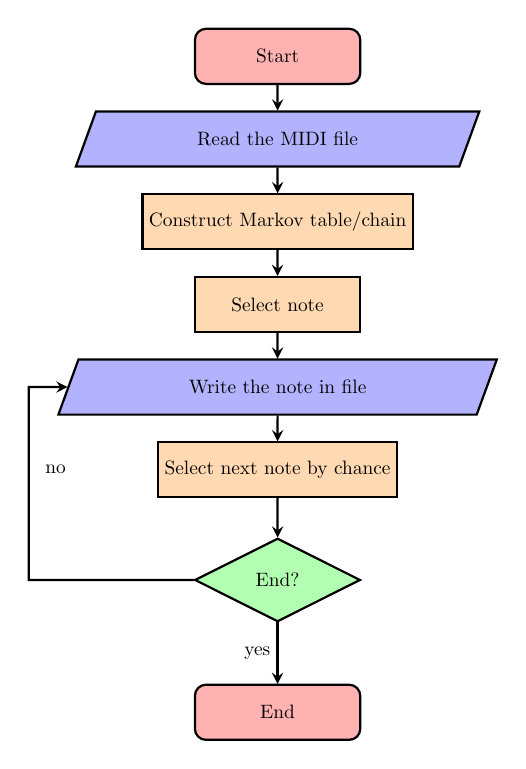
\begin{tikzpicture}[thick,scale=0.7, every node/.style={scale=0.7}, node distance=1.5cm]
                        \node (start) [startstop] {Start};
                        \node (in1) [io, below of=start] {Read the MIDI file};
                        \draw [arrow] (start) -- (in1);
                        \node (pro1) [process, below of=in1] {Construct Markov table/chain};
                        \draw [arrow] (in1) -- (pro1);
                        \node (pro2) [process, below of=pro1] {Select note};
                        \draw [arrow] (pro1) -- (pro2);
                        \node (out1) [io, below of=pro2] {Write the note in file};
                        \draw [arrow] (pro2) -- (out1);
                        \node (pro3) [process, below of=out1] {Select next note by chance};
                        \draw [arrow] (out1) -- (pro3);
                        \node (loop) [decision, below of=pro3, yshift=-0.5cm] {End?};
                        \draw [arrow] (pro3) -- (loop);
                        \draw [arrow] (loop.west) -- ++(-3,0) -- ++(0,1.75) -- ++(0,1.75) -- node[xshift=1.2cm,yshift=-1.5cm, text width=2.5cm] {no}(out1.west);
                        \node (end) [startstop, below of=loop, yshift=-0.9cm]{End};
                        \draw [arrow] (loop) -- node[anchor=east] {yes} (end);
                    \end{tikzpicture}
                    \caption{A common block diagram of the algorithms}
                \end{center}
            \end{figure}
            \subsubsection{Algorithm with one tune pitch}
            \paragraph{}This algorithm constructs a Markov table based only on the frequencies of the tones. The size of the table depends on the variety of tunes used. Then it selects starting note and each next note is picked using random number generator and the chances in the Markov chain.
            \subsubsection{Algorithm with one tune pitch and note duration}
            \paragraph{}This algorithm constructs a Markov table based on the frequencies of the tones and their length. Because of this the size of the table increases and the size depends ont only on the variety of notes but on the variety of note lengths. Then it selects starting note and each next note is picked using random number generator and the chances in the Markov chain.
            \subsubsection{Algorithm with two tune pitch}
            \paragraph{}This algorithm constructs a Markov table based only on the frequencies of the tones but it calculates the chance of next event, based ont he previous two, so the size of the table increases and is the size of the table in 1.4.1 sqared. Then it selects starting note and each next note is picked using random number generator and the chances in the Markov chain.
            \subsubsection{Rust}
            \paragraph{}All the implementations of the algorithms for the project are written in Rust programming language. It is based on C but it gaurantees memory safety, threads without data races, generics(templates) and the standart library is bigger and has some bindings for functional programming.
        \newpage
    \section{Results}
        \paragraph{}Here are listed some results. The tests are runned with original music ``Noctune op.9 no.2'' written by Chopin. Here is the music sheet of the piece(all the sheets are given in the github repo of the project like midi files):\\
        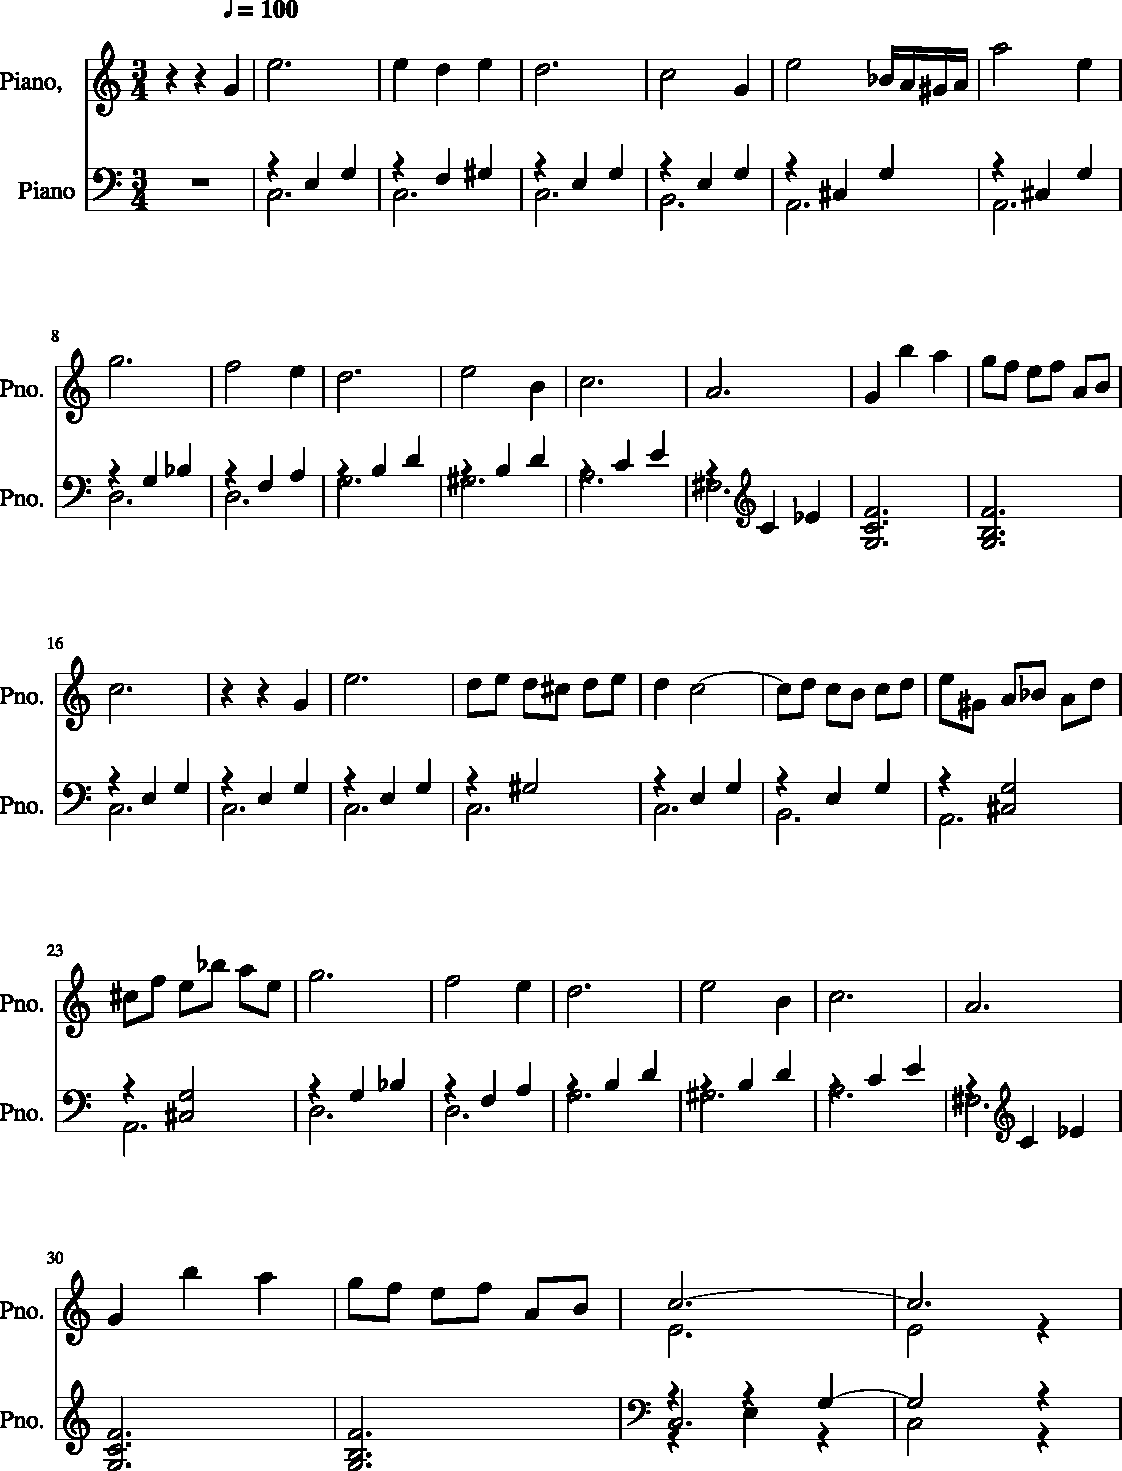
\includegraphics[scale=0.59]{original}\\
        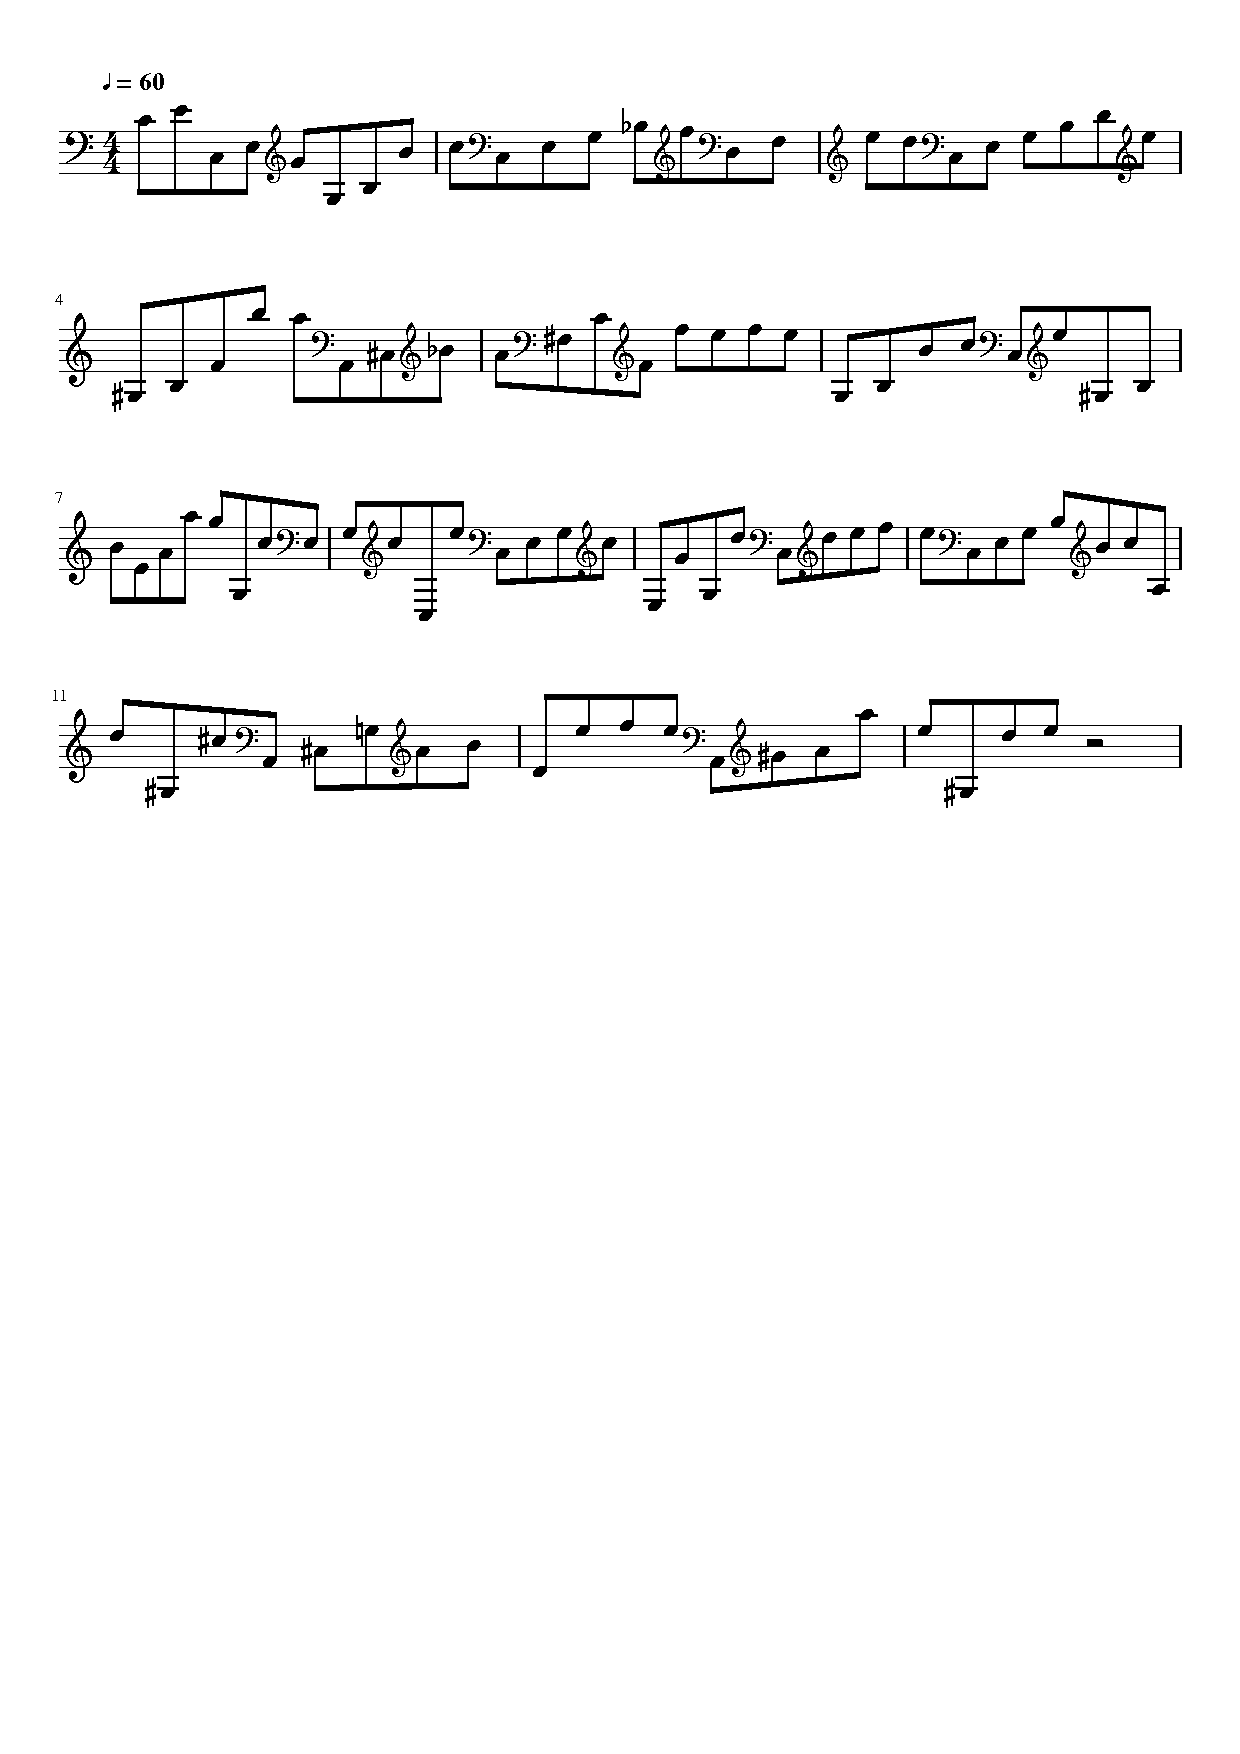
\includegraphics[scale=0.5]{result_one_note}
        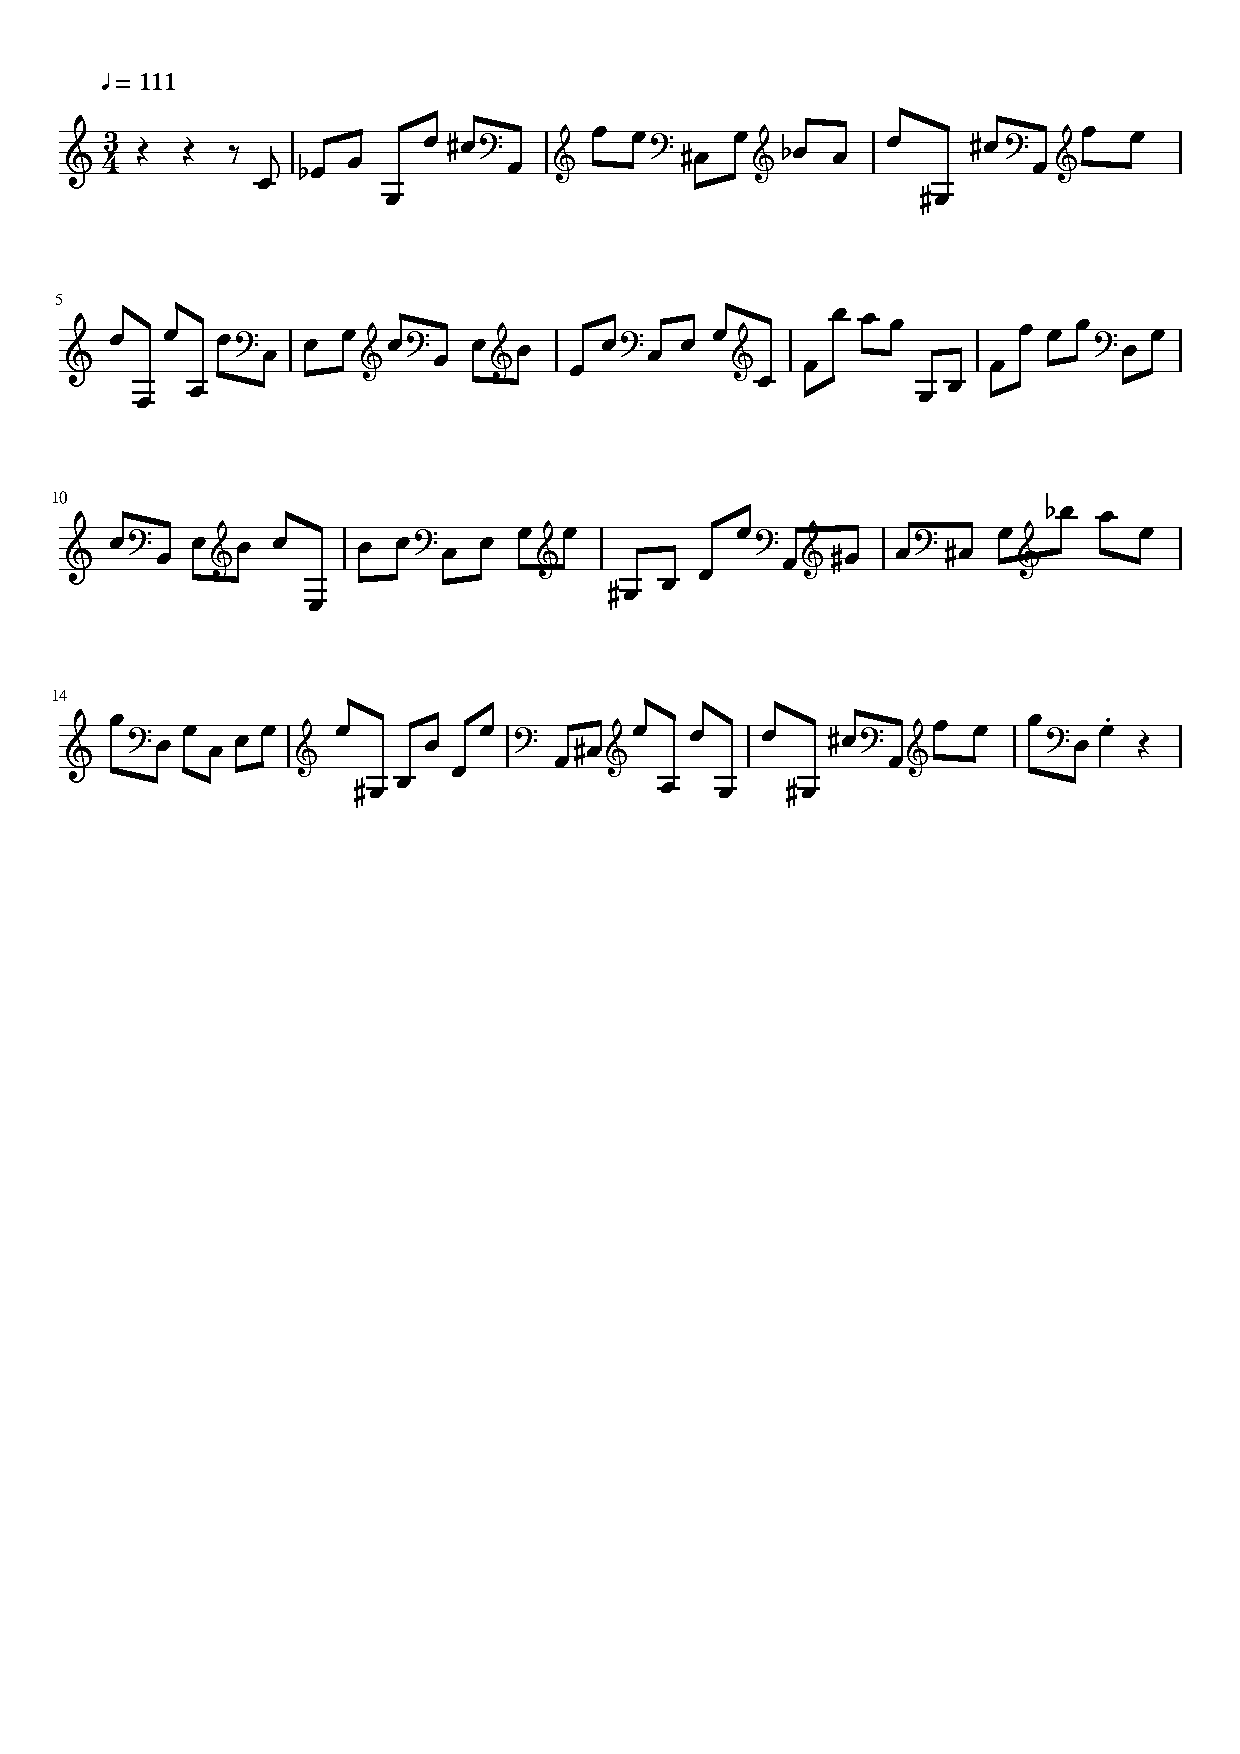
\includegraphics[scale=0.5]{result_one_note_time}
        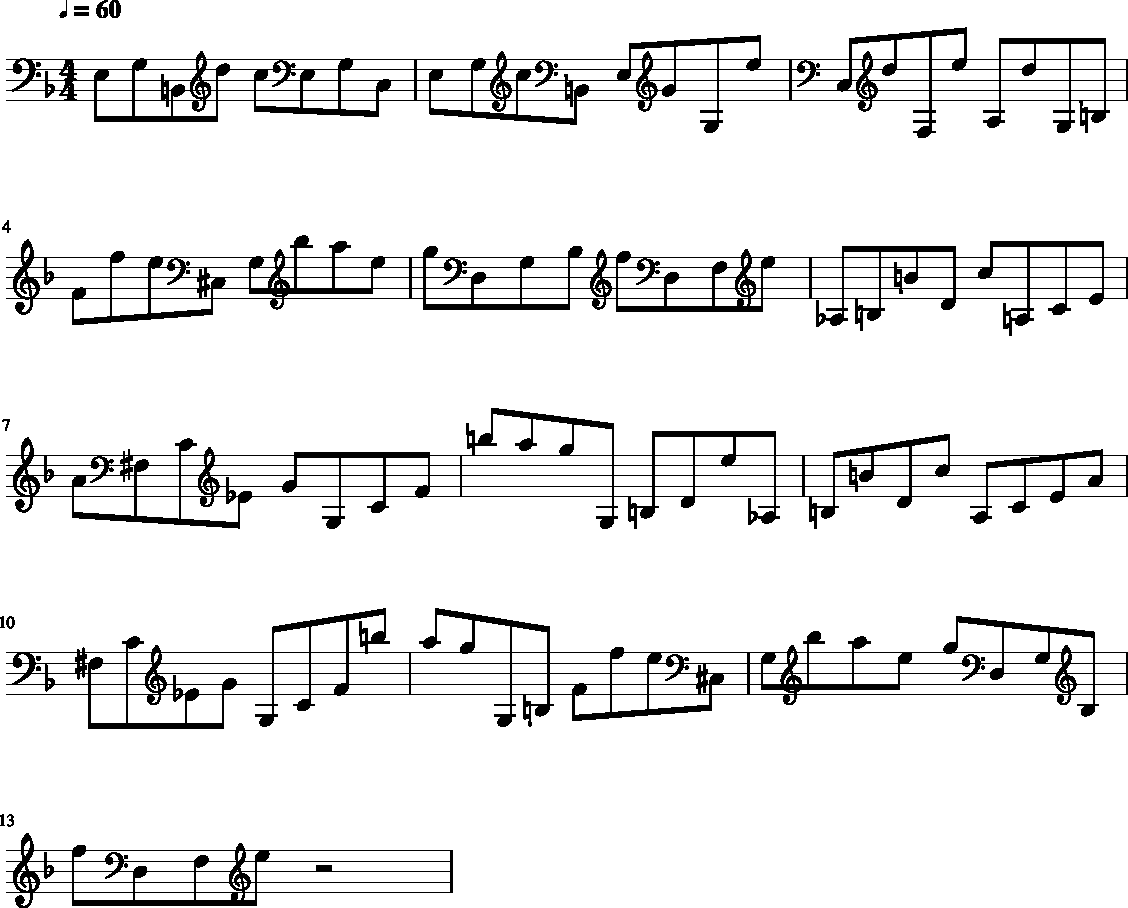
\includegraphics[scale=0.5]{result_pair_notes}
\end{document}